\documentclass{article}

\usepackage{here}
\usepackage{float}
\usepackage{adjustbox}
\usepackage{graphicx}
\usepackage{cite}
\usepackage{amsmath}
\usepackage{amssymb}
\usepackage{pifont}
\usepackage{enumitem}
\usepackage{url}
\usepackage{multirow}
\usepackage{etoolbox}
\usepackage{titlesec}
\newcommand{\cmark}{\ding{51}}

\DeclareMathOperator\erf{erf}

\interdisplaylinepenalty=2500
\hyphenation{op-tical net-works semi-conduc-tor}
\patchcmd{\thebibliography}{\section*{\refname}}{}{}{}
\setcounter{secnumdepth}{4}
\titleformat{\paragraph}
{\normalfont\normalsize\bfseries}{\theparagraph}{1em}{}
\titlespacing*{\paragraph}
{0pt}{3.25ex plus 1ex minus .2ex}{1.5ex plus .2ex}


\begin{document}

\title{The potential of a large dust grain in a collisionless plasma}
\author{Dogan Akpinar and George E. B. Doran}
\markboth{D. Akpinar \& G. E. B. Doran}
{Shell \MakeLowercase{\textit{et al.}}:}

\maketitle

\begin{abstract}

\end{abstract}

\section{Introduction}

\section{Background}

In the case of a large dust grain with a negative equilibrium charge, we can establish regions within an infinite plasma with well-defined
transitions. We firstly have the dust grain itself, followed
by a positive region of space, called the sheath, usually a few electron Debye lengths
in size. The electron Debye length is a characteristic length over which quasi-neutrality breaks down, 
defined as

\begin{equation}\label{eq:Debye}
\lambda_D = \sqrt{\frac{\varepsilon_{0} k_{B} T_{e}}{n_{0} e^2}},
\end{equation}

\smallskip

\noindent where $k_B$ is the Boltzmann constant, $T_e$ is the electron temperature, $e$ is the 
electron charge, $n_0$ is the electron number density at infinity and $\varepsilon_{0}$ is the
permittivity of free space. Following the sheath, we have the infinite pre-sheath where quasi-neutrality holds;
quasi-neutrality is mathematically written as an approximate equality between the ion and electron
densities, $Zn_i \approx n_e$.

\medskip

Positive ions are continuously collected by the negative dust, so there must be
a net influx of ions into the sheath to maintain the equilibrium. This established the Bohm
criterion, where the speed of ions required to enter the sheath must be 
greater then of equal to the Bohm speed. For the cold ion case, the Bohm speed is defined as

\smallskip 

\begin{equation}\label{eq:ColdBohm}
c_{s}^{cold} = \sqrt{\frac{k_{B}T_{e}}{m_{i}}},
\end{equation}

\noindent where $m_i$ is the ion mass and $c_{s}^{cold}$ is known as the cold ion Bohm speed. 
However, if we consider ions with a finite temperature, the required Bohm speed becomes 

\begin{equation}\label{eq:HotBohm}
c_{s}^{hot} = \sqrt{\frac{k_{B}(T_{e} + \gamma T_{i})}{m_{i}}},
\end{equation}

\smallskip

\noindent where $T_i$ is the ion temperature, $\gamma$ is the adiabatic index
and $c_{s}^{hot}$ is known as the hot ion Bohm speed \cite{Stangeby1986} \cite{Willis} .

\medskip

For a large dust grain, we may consider the planar sheath limit \cite{Willis}. 
Hence, the potential drop across the sheath for $T_i \neq 0$ is given as

\begin{equation}\label{eq:SheathDrop}
\phi_s = \frac{k_B T_e}{2e}\ln{\left[\frac{2\pi Z^2}{\mu^2}(1 + \gamma \Theta)\right]},
\end{equation}

\noindent where $Z$ is the relative ion charge, $\mu = \sqrt{\frac{m_i}{m_e}}$ and $\Theta = \frac{T_i}{T_e}$ \cite{Stangeby1986}.

\section{Radial motion theory (ABR)}

\smallskip

The ABR model is a radial motion theory derived by Allen, Boyd and Reynolds. It describes the equilibrium surface potential acquired
by a dust grain immersed in an infinite and stationary plasma \cite{ABR}.

\medskip

Consider a spherical dust grain, of arbitrary radius $a$, immersed in this infinite plasma. Far from the surface we assume that the electron
and ion densities are equal, denoted $n_e$ and $n_i$ respectively; this is known as quasi-neutrality. As electrons are faster than ions, it can be shown that such a dust grain will become negatively 
charged \cite{Thomas}, thus ions will experience an attractive force due to the potential on the dust surface, 
$\phi_a$. We assume that ions at infinity have no kinetic energy, hence, they move radially
towards the dust grain. Therefore, it is appropriate to say that an ion at a distance 
$r$ from the dust center has radial speed $v_i$. Using energy conservation, one can show the following,

\begin{equation}\label{eq:EnergyConservation}
\frac{1}{2} m_i v_i^2 = -Ze\phi(r),
\end{equation}

\noindent where $\phi(r)$ is the potential at $r$, which vanishes as $r \to \infty$ \cite{ABR}.

\medskip

Equation (\ref{eq:EnergyConservation}) then leads to an expression for the ion current, which is entirely dependant on the radial distance from the 
dust grain, given by

\begin{equation}\label{eq:ABRIi}
I_i = \frac{4\sqrt{2} \ n_i \pi r^2 Z^{\frac{3}{2}}e^{\frac{3}{2}} \phi_a^{\frac{1}{2}} } {m_i^{\frac{1}{2}}}.
\end{equation}

As the potential is negative, few electrons reach the dust grain, hence, the electron density obeys a Boltzmann
distribution:

\begin{equation}\label{eq:ABRed}
n_e(r) = n_0 \exp{\left(\frac{e\phi(r)}{k_B T_e}\right)},
\end{equation}

\smallskip

we further assume that only inbound electrons contribute to the electron current at the surface of the dust
grain, given as

\begin{equation}\label{eq:ABRIe}
I_i = I_e = 4 \pi a^2 n_0 e \sqrt{\frac{k_B T_e}{2 \pi m_e }} \exp{\left(\frac{e \phi_a}{k_B T_e}\right)}.
\end{equation}  

\noindent where $m_e$ is the electron mass \cite{ABR}.

\medskip

It is useful to apply the following normalisations, noting that $\Phi$ is the opposite
sign for simplicity:

\begin{equation}\label{eq:ABRnorm}
{\Phi = - \frac{e\phi}{k_B T_e}}, \ {\rho = \frac{r}{\lambda_D}},\ {\alpha = \frac{a}{\lambda_D}},\ {J = \frac{I_i}{4 \pi \lambda_D^2 n_0 e \sqrt{\frac{2k_B T_e}{m_i}}}},
\end{equation}
    
\noindent where $\lambda_D$ is the electron Debye length, 

\medskip

Poisson's law allows for the formation of a differential equation which relates
the spatial variation of the potential to the difference in electron and 
ion densities,

\begin{equation}\label{eq:ABR9} 
\frac{d}{d\rho} \left(\rho^2 \frac{d\Phi}{d\rho}\right) = J Z^{-\frac{1}{2}}\Phi^{-\frac{1}{2}}  - \rho^2 \exp{(-\Phi)}.
\end{equation}

\medskip

\noindent This equation may be solved using the boundary conditions;

\begin{equation}\label{eq:ABR10}
\rho \approx J^{\frac{1}{2}} Z^{-\frac{1}{4}} \Phi^{-\frac{1}{4}} \exp{\left(\frac{\Phi}{2}\right)},
\end{equation}
 
\begin{equation}\label{eq:ABR11}
\frac{d\Phi}{d\rho}\biggr|_{\rho_b} = \frac{2\rho_b Z^{\frac{1}{2}} J^{-1} \Phi_b^{\frac{3}{2}}}{\Phi_b - \frac{1}{2}} exp{(-\Phi_b)},
\end{equation}
 
\begin{equation}\label{eq:ABR13}
\frac{J}{\Gamma} = \frac{4Z^{\frac{1}{2}}\Phi_b^{\frac{3}{2}}(2\Phi_b - 3)(2\Phi_b + 1)}{(2\Phi_b - 1)^3},
\end{equation}

\begin{equation}\label{eq:ABR12}
\frac{J}{\alpha^2} = \frac{\mu}{\sqrt{4\pi}} \exp{\left(-\Phi_a\right)},
\end{equation}

\medskip

\noindent which are formed by assuming that there exists a certain distance $\rho_b$, past which, quasi-neutrality applies. 
The potential at $\rho_b$ is given by $\Phi_b$, and $\Gamma$ is a number much greater than unity \cite{ABR}.
In order to find a value for the surface potential we must solve (\ref{eq:ABR9}), this may be 
achieved using a 4th order Runge-Kutta. We choose $\Gamma = 10000$ and find the roots of 
(\ref{eq:ABR13}) allowing us to determine the necessary boundary conditions 
using (\ref{eq:ABR10}) and (\ref{eq:ABR11}). Hence, solving the differential equation numerically, yields 
the following graph of normalised dust potential as a function of normalised dust radius.

\begin{figure}[H]
\centering
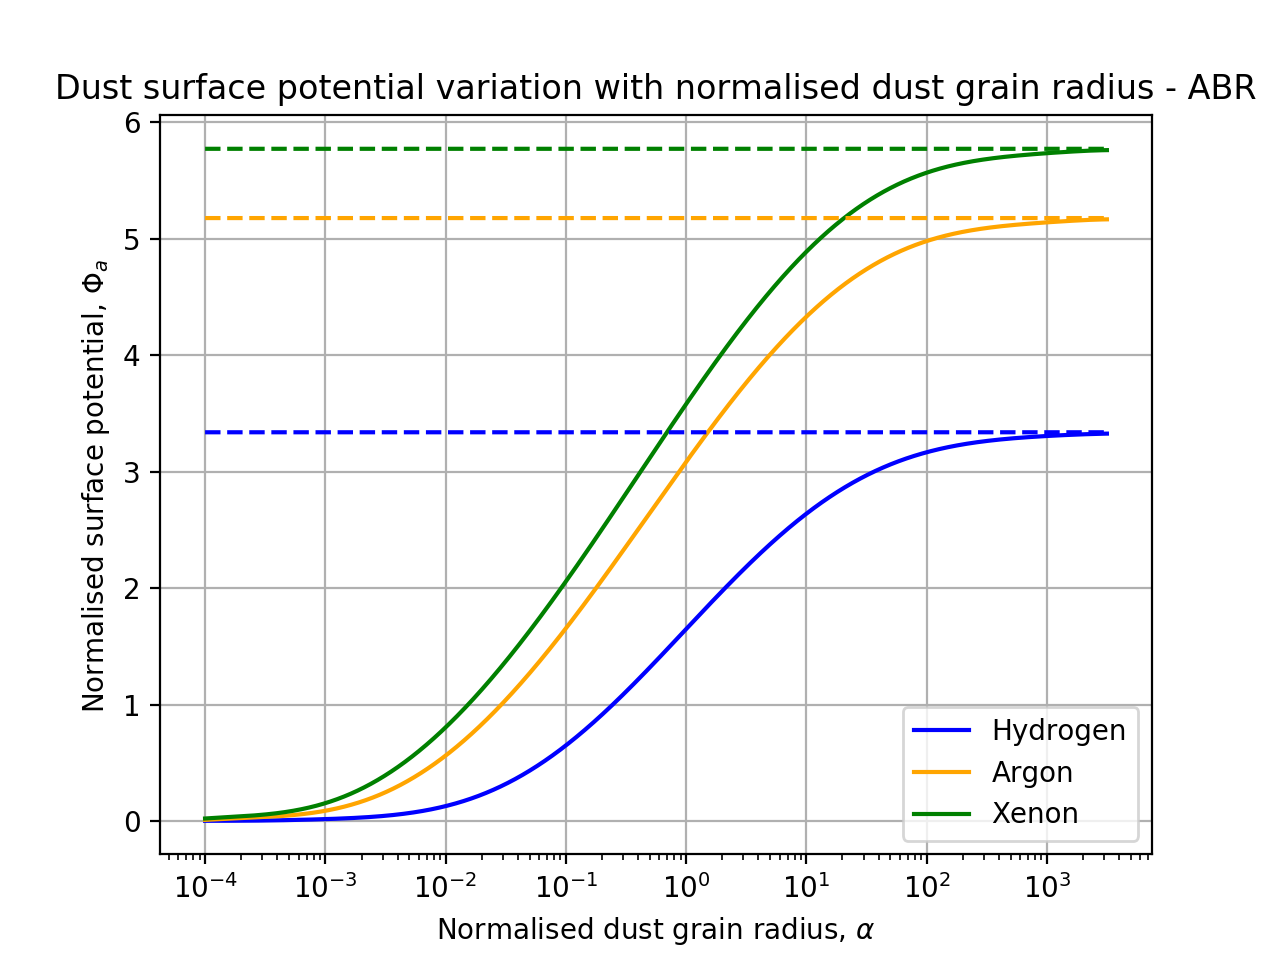
\includegraphics[width=\linewidth]{Output/ABRgraph.jpeg}
\caption{ABR predictions for $\Phi_a$ as a function of $\alpha$ for a dust grain in singly ionised Hydrogen, Argon and Xenon plasmas ($Z=1$) \cite{ABR} \cite{Thomas}.}
\label{ABR} 
\end{figure}

Thomas discusses that in the limit of $\alpha \to \infty$ the ABR potential approaches
the cold planar wall limit \cite{Thomas}, given as the following 

\begin{equation}\label{eq:ABRLim}
\lim_{\alpha \to \infty} \Phi_a = \frac{1}{2}\ln{\left(2 \pi \right)} - \frac{1}{2} - \ln{\left(\mu \right)},
\end{equation}

\smallskip

\noindent where $Z = 1$ and the $-\frac{1}{2}$ is due to the potential drop across the cold ion pre-sheath,
as discussed by Stangeby \cite{Stangeby1986} \cite{Stangeby2000}. Furthermore, one can clearly see that in the limit
of $\alpha \to 0$ the ABR prediction tends to zero also \cite{ABR}.

\section{Modified orbital motion limited (MOML)}

\smallskip

Orbital motion limited (OML) is known to model the potential on a small spherical
dust grain immersed in an infinite and collisionless plasma, it does so by considering
energy and angular momentum conservations of ions along side a critical grazing incidence.
OML considers an equilibrium of ion and electron currents at the dust 
surface, $I_i = I_e$, while simultaneously invoking quasi-neutrality.
Hence, the standard result acquired from OML is 
the following

\begin{equation}\label{eq:OMLeqn}
\frac{\sqrt{\Theta}}{\mu} \left(1 - \frac{Z}{\Theta}\Phi_a \right) \approx \exp{\left(\Phi_a\right)}.
\end{equation}

\medskip

Using available OM data, Willis discusses that any error in OML is negligible for small dust grains,
he further proposes an upper radius limit for OML which is $\Theta$ dependant \cite{Willis}. Furthermore, it should be noted that
OML guarantees the existence of absorption radii, $r_{A} > a$, such that any 
ion within $r_{A}$ approaching the dust grain will be collected \cite{Thomas}. 

\medskip

In order to model a large dust grain, we must slightly change our approach to the problem.
We now apply OML to the boundary between the sheath and pre-sheath, this establishes
the assumption that as $\alpha \to \infty$ any ion that enters the sheath will be 
collected by the dust grain. For such dust grains, of large radii, the majority of absorption
radii occur within the sheath, hence, applying OML in this was eliminates most of the inaccuracies introduced 
by absorption radii and ensures the validity of MOML. However, it will be shown later that the validity of MOML in fact breaks down for small
on $\Theta$ \cite{Thomas}. 

\medskip

Replacing $\Phi_a$ on the left hand side in (\ref{eq:OMLeqn}) with $\Phi_s$ physically amounts to
saying that as $\alpha \to \infty$, all ions that enter the sheath are absorbed. Considering an equilibrium of
electron and ion currents at the sheath edge while simultaneously invoking quasi-neutrality 
and the expression for the hot ion Bohm speed, (\ref{eq:HotBohm}), one acquires the following 
relationship between $\Phi_s$ and $\Phi_a$

\begin{equation}\label{eq:PhiS}
\Phi_s \approx \Phi_a - \frac{1}{2}\ln{\left[\frac{2\pi Z^2}{\mu^2}(1 + \gamma \Theta)\right]},
\end{equation}

\noindent where the second term is the normalised sheath potential drop, (\ref{eq:SheathDrop}).
Substituting (\ref{eq:PhiS}) into the modified (\ref{eq:OMLeqn}) and manipulating in terms of
the the principle branch of the Lambert W function, $W_0$, yields 

\begin{equation}\label{eq:MOMLsol}
\Phi_a \approx  \frac{\Theta}{Z} - W_{0}\left(\sqrt{2\pi \Theta (1 + \gamma \Theta)} \exp{\left (\frac{\Theta}{Z}\right)}\right) + \frac{1}{2}\ln{\left[\frac{2\pi Z^2}{\mu^2}(1 + \gamma \Theta)\right]}.
\end{equation}

Willis compares the MOML solution with simulated data ran by PIC and concludes that 
$\gamma = \frac{5}{3}$ seems to produce the most appropriate predictions \cite{Willis}. 
Hence, $\gamma = \frac{5}{3}$ is chosen as the default value for our investigation. It is worth noting
that from (Fig. \ref{MOMLgamma}) we see that for extreme $\Theta$ values, 
the choice of $\gamma$ has very little affect on the predicted potential; the same can be said for 
intermediate values of $\Theta$ as there is very little difference in the predicted potentials for 
each $\gamma$ value. 

\begin{figure}[H]
\centering
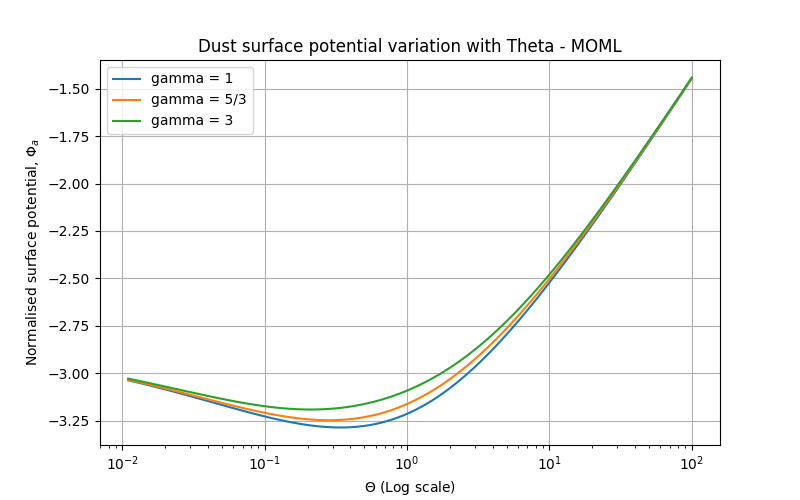
\includegraphics[width=\linewidth]{Output/MOMLgamma.jpeg}
\caption{The MOML prediction for  $\Phi_a$ as a function of $\Theta$, for a hydrogenic ($\mu \approx 43$) and singly ionised ($Z = 1$) plasma with different values of $\gamma$ \cite{Thomas}.}
\label{MOMLgamma} 
\end{figure}


\begin{figure}[H]
\centering
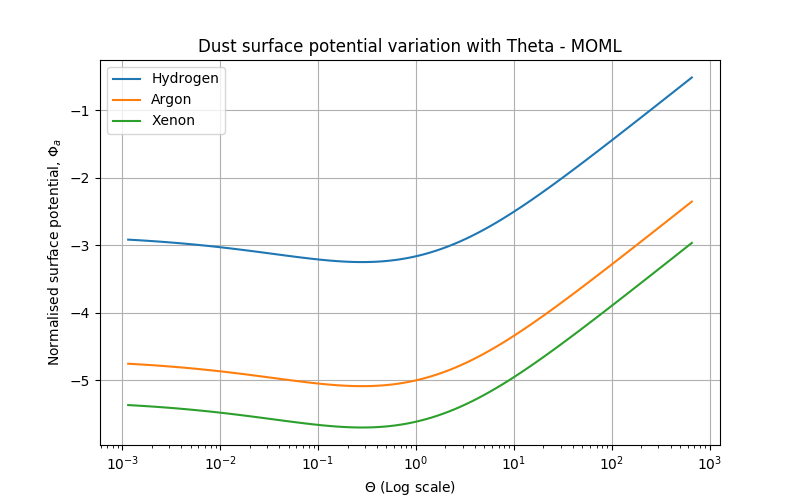
\includegraphics[width=\linewidth]{Output/MOMLgraph.jpeg}
\caption{Normalised surface potential as a function of $\Theta$ for singly ionised ($Z = 1$) Hydrogen, Argon and Xenon plasmas according on the MOML prediction, plotted on a log-linear scale. The normalised surface potential progressively becomes more negative as the ion species becomes heavier \cite{Thomas}.}
\label{MOMLgraph} 
\end{figure}
    
    
\section{SCEPTIC numerical fit}
\section{Comparison of MOML and ABR with SCEPTIC data}
\section{Flowing sheath approximation}
\section{Conclusion}


\section{References and Acknowledgements}
\bibliography{DustyLib}
\bibliographystyle{IEEEtran}

\section{Appendix}

\subsection{Symbol dictionary}
\begin{center}
\begin{tabular}{cl} 

$e$ & Electron charge \\
$\varepsilon_0$ & Permittivity of free space \\
$k_B$ & Boltzmann's constant \\
$a$ & Dust radius\\
$\alpha$ & Normalised dust radius \\
$_a$ & Subscript indicating a quantity at the dust grain surface \\
$r$ & Distance from the centre of the dust grain \\
$\rho$ & Normalised distance from the centre of the dust grain \\
$\lambda_D$ & Debye length \\
$m_j$ & Mass \\
$n_j$ & Density \\
$T_j$ & Temperature \\
$I_j$ & Current \\
$_j$ & Subscript indicating a plasma particle \\
$_i$ & Subscript indicating an ion quantity \\
$_e$ & Subscript indicating an electron quantity \\
$_0$ & Subscript indicating an electron quantity at infinity \\
$\mu$ & Root mass ratio\\
$\Theta$ & Ratio of ion to electron temperature \\
$\gamma$ & Heat capacity ratio \\
$u$ & Flow velocity \\
$\upsilon$ & Normalised flow velocity \\
$\Gamma$ & ABR correction factor \\
$Z$ & Ion charge number \\
$Q$ & Dust grain charge \\
$\phi$ & Electric potential \\
$\Phi$ & Normalised electric potential \\

\end{tabular}
\end{center}



\end{document}